\section{Introdução}

% Bluetooth Overview
Bluetooth é uma tecnologia de comunicação sem fio de curto alcance desenvolvida
pelo BLuetooth Special Interest Group, também conhecido como Bluetooth SIG. Esta
tecnologia está presente em uma vasta gama de dispositivos, sendo utilizada em
smartphones, computadores, automóveis, tablets entre
outros\cite{gomez2012overview}.

O Bluetooth Low Energy, ou BLE, é uma das formas de operação previstas na
especificação da versão 4.0 do Bluetooth. Junto com o BLE, o documento também
especifica a operação do tipo Basic Rate, também chamado de BR, dando
continuidade as formas de operação definidas nas versões anteriores do bluetooth.\cite{ble4core}.
Um dispositivo bluetooth pode operar na forma Single Mode, sendo compatível
apenas com BLE, ou na forma Dual Mode, sendo compatível com as duas
formas de operação. \cite{ble4core}.

% O que o BLE faz para ser Low Power

Um dispositivo BLE pode operar de 4 formas diferentes: Broadcaster, Observer,
Slave e Central. \cite{ble4core}.

Como Broadcaster, o dispositivo opera somente como transmissor de dados,
enviando pacotes de dados periodicamente, ação denominada Advertising, que
podem conter informações sobre o dispositivo e indicam a presença de um 
dispositivo num dado local. Quando um dispositivo opera apenas como
broadcaster, ele não está aberto a receber conexões.\cite{ble4core}.

Como Observer, o dispositivo opera somente como um receptor de dados, recebendo
apenas os pacotes de advertising enviados por outros dispositivos
BLE.\cite{ble4core}.

Como Peripheral, o dispositivo suporta estabelecer uma conexão como slave. Para
outro dispositivo detectar sua presença e iniciar uma conexão, é necessário que
o peripheral opere antes como um broadcaster, indicando sua
presença.\cite{ble4core}.

Como Central, o dispositivo suporta múltiplas conexões como master e é sempre o
responsável por iniciar as conexões com um peripheral. Para detectar um
peripheral, é necessário que a central opere como um observer para detectar a
presença de outros dispositivos.\cite{ble4core}. Um dispositivo é capaz de
suportar múltiplas formas de operação ao mesmo tempo.\cite{ble4core}.

% Descrição do meio físico
O BLE opera na frequência de 2.4GHz utilizando 40 canais de 2MHz com
frequências de centro de 2402MHz a 2480MHz. Existem dois tipos de transmissão: a
transmissão de dados, que é feita em 37 dos canais disponíveis com a capacidade
de transmissão de 1Mbit/s, que é realizada pelos dispositivos operando como
central ou como peripeheral; e o Advertising, que é feito nos outros 3 canais
restantes com as frequências de 2402MHz, 2426MHz e 2480MHz, que
é realizado nos dispositivos operando como broadcaster.\cite{ble4core}

A tabela \ref{tab:adv_channel_list} mapeia os canais de rádiofrequência para os canais
utilizados pelo BLE com suas respectivas identificações e finalidades. 	

\begin{center}
	\centering 
	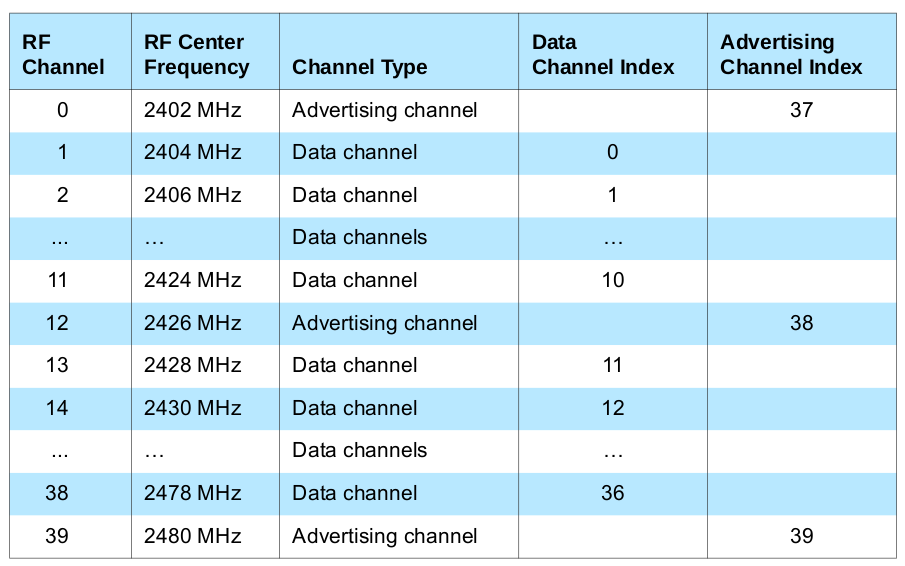
\includegraphics[width=0.8\linewidth]{adv_ch_map.png}
	\captionof{table}{Mapeamento dos canais de RF para os canais do BLE \cite{ble4core}}
	\label{tab:adv_channel_list}
\end{center} 
 
Advertising é a ação de transmitir pacotes de dados de forma pública para todos
os dispositivos capazes de recebê-los nos três canais de advertising, com a
finalidade principal de indicar a presença do dispositivo no local e é
realizada pelos dispositivos que operam como periperal ou como broadcaster
\cite{ble4core}. Logo após o envio de um pacote de advertising em um  canal, o
broadcaster fica apto a receber uma mensagem por um instante, e quando um
peripheral ou central recebem um advertising, podem ser solicitadas mais
informações nesse mesmo instante através da transmissão de um pacote de Scanner
Request que é enviado, e quando o broadcaster recebe esta solicitação um pacote
chamado Scan Response é enviado.

Durante este instante em que o broadcaster pode receber uma solicitação, é
possível também que uma central faça uma solicitação de início de conexão,
portanto, uma conexão só pode ser iniciada no envio de um pacote de advertising. 

Os pacotes de advertising podem
ser conectáveis ou não conectáveis.
Quando um observer ou uma central detectam um pacote de advertising é possível solicitar mais informações do
dispositivo através do Scanner Request, 

 transmitir um comando sem a
necessidade de estabelecer uma conexão

% Os canais de Advertising possuem, frequências estratégicas para evitar
% interferências causadas pela coexistência do BLE com redes Wi-Fi, como 
% mostra a figura \ref{fig:wifi_coexist}
% 
% \begin{center}
% 	\centering 
% 	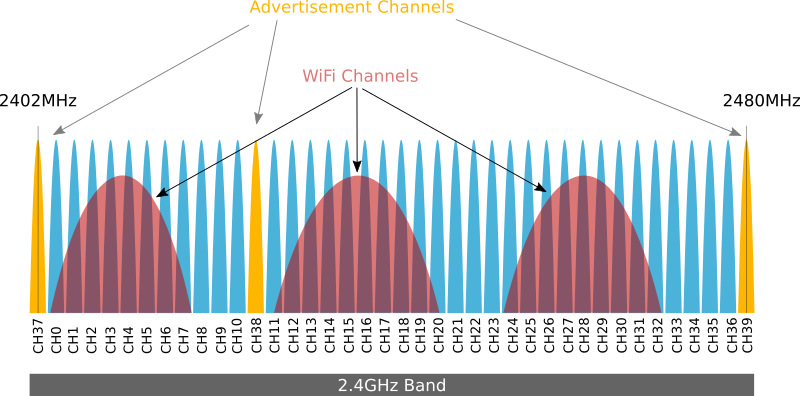
\includegraphics[width=0.85\linewidth]{ble-advertising-channels-spectrum.png}
% 	\captionof{figure}{Coexistência entre BLE e Wi-Fi}
% 	\label{fig:wifi_coexist}
% \end{center} 
% 
% 

Um dispositivo BLE pode possuir 4 formas distintas de operação

% GAP
    %Profiles
    
    

Na função de Broadcaster, o dispositivo opera apenas transmitindo pacotes de dados periodicamente nos três canais de advertising. 
Estes pacotes de dados, além de indicar a presença do dispositivo, contém os dados que são formatados de acordo com as especificações do BLE. 
Existem dois tipos de pacotes que o Broadcaster envia, que pode ser o advertising, pacote transmitido periodicamente, ou scan response,
que é o pacote transmitido quando um Observer detecta um advertising e solicita outro pacote com mais informações.

Já na função de Observer o dispositivo opera apenas lendo dados Nestas duas
funções o fluxo de dados é unidirecional.
    
Na função de Peripheral o dispositivo é capaz de estabelecer conexões com
outros dispositivos, porém operando num modo slave sendo controlado através de
um dispositivo master. A quarta função é a central Bluetooth, que pode operar tanto com.

    % Serviços e caracteríscas

    % tipos de mac: vol 6 part B 1.3.2
No BLE os dispositivos são identificados através do Device Address, ou Endereço
do Dispositivo, que possui 48 bits. O endereço do dispositivo também é chamado
de MAC Address. Existem dois tipos de endereço: o endereço público e o
aleatório.


% Link layer

%% definir GAP

% O Bluetooth Low Energy, ou BLE, é uma das formas de operação previstas na
% especificação da versão 4.0 do Bluetooth.
% Junto com o BLE, o documento também especifica a operação do tipo Basic Rate,
% compatibilizando a versão 4.0 com as versões anteriores.


% Topologia:

% No BLE os dispositivos podem assumir 4 funções diferentes. São elas: Broadcaster, Observer, Peripheral e Central.
% Na função de Broadcaster, o dispositivo opera apenas transmitindo dados. Já na função de Observer o dispositivo opera apenas lendo dados Nestas duas funções o fluxo de dados é unidirecional.
% Na função de Peripheral o dispositivo é capaz de estabelecer conexões com outros dispositivos, porém operando num modo slave sendo controlado através de um dispositivo master. A quarta função é a central Bluetooth, que pode operar tanto com.

% Operação:

% O rádio do BLE opera na frequência de 2.4GHz utilizando a técnica de frequency hopping para combater interferência de muitas portatoras FHSS.

% São utilizados dois tipos de acesso: FDMA e TDMA. Existem 40 canais físicos separados por 2MHz utilizando a técnica FDMA. Entre esses canais, 37 são usados como canais de dados e 3 são canais utilizados para advertising.

% Aplicações:


